\documentclass[11pt,a4paper]{article}

\usepackage[utf8]{inputenc}
\usepackage[T1]{fontenc}
\usepackage{lmodern}
\usepackage[margin=2.2cm]{geometry}
\usepackage{amsmath,amssymb,mathtools,bm}
\usepackage{booktabs,tabularx,longtable,array}
\usepackage{enumitem}
\usepackage[raggedright]{titlesec}
\usepackage{xcolor}
\usepackage{hyperref}
\usepackage{tikz}
\usetikzlibrary{arrows.meta,positioning,fit,backgrounds,calc}

\hypersetup{
    colorlinks=true,
    linkcolor=blue!60!black,
    urlcolor=blue!60!black,
    citecolor=blue!60!black
}

\newcolumntype{L}[1]{>{\raggedright\arraybackslash}p{#1}}
\newcolumntype{C}[1]{>{\centering\arraybackslash}p{#1}}
\newcolumntype{Y}{>{\raggedright\arraybackslash}X}

\newcommand{\importantbox}[2]{%
  \par\medskip\noindent
  \fcolorbox{blue!50!black}{blue!4!white}{%
    \parbox{\dimexpr\linewidth-2\fboxsep-2\fboxrule\relax}{%
      \textbf{#1}\par\smallskip #2%
    }%
  }\par\medskip
}

\setlength{\parskip}{0.45em}
\setlength{\parindent}{0pt}

\title{\textbf{Atom-to-Reactor: Two-Dimensional Composition Grid, Solvation Models, and Fitting vs.\ Prediction}}
\author{Department of Chemistry -- \AA ngstr\"om Laboratory, Uppsala University}
\date{}

\begin{document}
\sloppy
\maketitle

This note specifies how the three design choices---water content, $\text{EC}/\text{DEC}$ solvent ratio, and thermodynamic solvation vector ($\Delta E_{\text{solv}, i}$)---enter the thermodynamic and kinetic calculations, and explains how kinetic fitting loops uniformly over every solvation vector (computed or experimentally fitted) across the kinetic structures (\texttt{M1}, \texttt{M1-split}) and the $5 \times 5$ composition grid.

\section{The Three Specification Axes}

When exploring the two-dimensional composition space together with the solvation description, three quantities are specified:

\begin{enumerate}[leftmargin=1.8em]
    \item \textbf{Water content ($\text{vol}\%\ \text{H}_2\text{O}$):}
    \[
        \text{water} \in \{0,\; 0.5,\; 1.0,\; 1.5,\; 2.0\}\;\text{vol}\%
    \]
    Added to the solvent before $\text{TMSPA}$ ($5\;\text{vol}\%$ by default). It sets the initial concentration $[\text{H}_2\text{O}]_0$ and slightly dilutes $[\text{TMSPA}]_0$ and $[\text{EC}]_0$, while leaving all standard-state reaction free energies $\Delta G_{\text{rxn}, j}^\circ$ unchanged.

    \item \textbf{Solvent ratio ($\text{DEC}$ volume fraction $f_{\text{DEC}}$):}
    \[
        f_{\text{DEC}} \in \{0,\; 0.25,\; 0.50,\; 0.75,\; 1.00\} \qquad (x_{\text{EC}}^\circ = 1 - f_{\text{DEC}})
    \]
    Here $f_{\text{DEC}} = 0$ is neat $\text{EC}$ and $f_{\text{DEC}} = 1$ is neat $\text{DEC}$. The solvent ratio acts on \emph{both} thermodynamics and kinetics:
    \begin{itemize}[leftmargin=1.5em]
        \item It mixes the neat-$\text{EC}$ and neat-$\text{DEC}$ solvation energies $\Delta E_{\text{solv}, i}$ by solvent mole fraction ($x_{\text{EC}}, x_{\text{DEC}}$), shifting $\Delta G_{\text{rxn}, j}^\circ$, $K_{\text{eq}, j}$, and every Marcus barrier $\Delta G_{f, j}^\ddagger$.
        \item It scales the initial ethylene carbonate concentration $[\text{EC}]_0$ available for solvent attack ($\text{R8}$--$\text{R9}$), from $[\text{EC}]_0 \approx 14.2\;\text{M}$ at $f_{\text{DEC}} = 0$ (with $5\;\text{vol}\%\ \text{TMSPA}$ and $2\;\text{vol}\%\ \text{H}_2\text{O}$) through $7.1\;\text{M}$ at $f_{\text{DEC}} = 0.50$, down to $0\;\text{M}$ at $f_{\text{DEC}} = 1$.
    \end{itemize}

    \item \textbf{Thermodynamic solvation vectors (\texttt{thermo\_models}, matching \texttt{solvset.py}):}
    Solvation inputs are organized in a two-level hierarchy of families (\texttt{thermo\_models}) and concrete instances (snapshots or equilibrium fits), with gas-phase $\Delta G_{\text{gas}, i}^\circ$ from $\omega\text{B97M-V}$ fixed across all of them:
    \begin{align*}
        \texttt{thermo\_models} &= (\texttt{MD},\; \texttt{COSMO},\; \texttt{Experimental}) \\
        \texttt{MD} &= [\texttt{snapshot\_1}\ (\texttt{2026-10-08}),\; \texttt{snapshot\_2}\ (\texttt{2026-11-12}),\; \dots] \\
        \texttt{COSMO} &= [\texttt{cosmors},\; \dots] \\
        \texttt{Experimental} &= [\texttt{exp\_1}\ (\texttt{thermo2\_2pctH2O}),\; \texttt{exp\_2}\ (\texttt{thermo4\_2pct\_cosmors}),\; \dots]
    \end{align*}
    Once the \texttt{Experimental} fits have been obtained from equilibrium NMR spectra, every \texttt{(thermo\_model, instance)} pair resolves to a species solvation vector $E_{\text{solv}, i}$ \textbf{on the exact same footing}. Computed vectors (\texttt{MD}, \texttt{COSMO}) and fitted vectors (\texttt{Experimental}) are interchangeable $E_{\text{solv}}$ data vectors for all downstream kinetic fits and grid evaluations.
\end{enumerate}

\begin{table}[h!]
\centering
\small
\begin{tabularx}{\linewidth}{@{}L{2.1cm}L{4.4cm}L{2.8cm}Y@{}}
\toprule
\textbf{\texttt{thermo\_model}} & \textbf{Instance (\texttt{snapshot}/\texttt{fit})} & \textbf{Source of $E_{\text{solv}}$ vector} & \textbf{Description} \\
\midrule
\texttt{MD} & \texttt{snapshot\_1} (\texttt{2026-10-08}) & Pure MACE MD & Computed MD solvation vector from the initial snapshot ($\delta = 0$) \\
\texttt{MD} & \texttt{snapshot\_2} (\texttt{2026-11-12}) & Pure MACE MD & Computed MD solvation vector from the updated campaign ($\delta = 0$) \\
\texttt{COSMO} & \texttt{cosmors} & Pure openCOSMO-RS & Computed continuum solvation free energy $\Delta G_{\text{solv}, i}$ ($\delta = 0$) \\
\texttt{Experimental} & \texttt{exp\_1} (\texttt{thermo2\_2pctH2O}) & \texttt{2026-10-08} MD + $\delta$ & MD vector shifted within $\pm\xi\sigma$ by equilibrium $2\%\ \text{H}_2\text{O}$ ($\text{EC:DEC } 1:1$) fit \\
\texttt{Experimental} & \texttt{exp\_2} (\texttt{thermo4\_2pct\_cosmors}) & \texttt{COSMO} + $\delta$ & COSMO vector shifted within $\pm\xi\sigma$ by equilibrium $2\%\ \text{H}_2\text{O}$ ($\text{EC:DEC } 1:1$) fit \\
\bottomrule
\end{tabularx}
\end{table}

\importantbox{Assumption when extrapolating \texttt{Experimental} vectors across $f_{\text{DEC}}$}{%
The species shifts $\delta E_{\text{solv}, i}$ in \texttt{exp\_1} and \texttt{exp\_2} were fitted at $f_{\text{DEC}} = 0.50$ ($\text{EC:DEC } 1:1$). When evaluated at any other $f_{\text{DEC}}$, the underlying computed medium mixes the neat-$\text{EC}$ and neat-$\text{DEC}$ values while the shifts $\delta E_{\text{solv}, i}$ are carried over unchanged as a constant species offset.}

\section{Sequential Pipeline and All-vs-All Comparison Matrix}

In the standard workflow, thermodynamics and kinetics are \textbf{not} fitted simultaneously. Equilibrium NMR data produces \texttt{Experimental} $E_{\text{solv}}$ vectors that sit on the exact same level as computed \texttt{MD} and \texttt{COSMO} vectors. Downstream kinetic fitting then runs identically over \emph{every} $E_{\text{solv}}$ vector and \emph{every} kinetic structure so that everything can be compared against everything:

\begin{center}
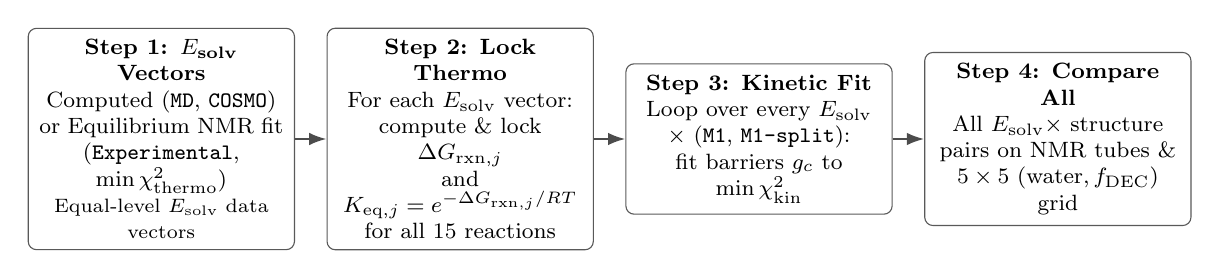
\begin{tikzpicture}[
    box/.style={draw=black!65, rounded corners=3pt, fill=white, align=flush center,
        font=\footnotesize, inner sep=4pt, text width=3.1cm},
    arr/.style={-{Latex[length=2.2mm,width=1.6mm]}, thick, draw=black!70}
]
\node[box] (S1) {\textbf{Step 1: $E_{\text{solv}}$ Vectors}\\Computed (\texttt{MD}, \texttt{COSMO})\\or Equilibrium NMR fit\\(\texttt{Experimental}, $\min \chi^2_{\text{thermo}}$)\\{\scriptsize Equal-level $E_{\text{solv}}$ data vectors}};
\node[box, right=0.4cm of S1] (S2) {\textbf{Step 2: Lock Thermo}\\For each $E_{\text{solv}}$ vector:\\compute \& lock $\Delta G_{\text{rxn}, j}$\\and $K_{\text{eq}, j} = e^{-\Delta G_{\text{rxn}, j}/RT}$\\for all 15 reactions};
\node[box, right=0.4cm of S2] (S3) {\textbf{Step 3: Kinetic Fit}\\Loop over every $E_{\text{solv}}$\\$\times$ (\texttt{M1}, \texttt{M1-split}):\\fit barriers $g_c$ to $\min \chi^2_{\text{kin}}$};
\node[box, right=0.4cm of S3] (S4) {\textbf{Step 4: Compare All}\\All $E_{\text{solv}} \times$ structure\\pairs on NMR tubes \&\\$5 \times 5$ $(\text{water}, f_{\text{DEC}})$ grid};
\draw[arr] (S1) -- (S2);
\draw[arr] (S2) -- (S3);
\draw[arr] (S3) -- (S4);
\end{tikzpicture}
\end{center}

\begin{enumerate}[leftmargin=1.8em]
    \item \textbf{Step 1 --- Assemble equal-level $E_{\text{solv}}$ vectors:} Each \texttt{(thermo\_model, instance)} yields a fixed species solvation vector $E_{\text{solv}, i}$:
    \begin{itemize}[leftmargin=1.5em]
        \item For \texttt{MD} and \texttt{COSMO}, $E_{\text{solv}, i}$ is taken directly from the quantum/MD calculation (no equilibrium fitting).
        \item For \texttt{Experimental}, equilibrium NMR points only are used to fit $\delta E_{\text{solv}, i}$ inside $\pm \xi\,\sigma_{\text{solv}, i}$ minimizing $\chi^2_{\text{thermo}}$; once fitted, the resulting $E_{\text{solv}, i} = E_{\text{solv}, i}^{\text{base}} + \delta E_{\text{solv}, i}$ becomes a fixed $E_{\text{solv}}$ data vector at the exact same level as \texttt{MD} and \texttt{COSMO}.
    \end{itemize}
    \item \textbf{Step 2 --- Lock $\Delta G_{\text{rxn}, j}$ and $K_{\text{eq}, j}$ for each vector:} From each $E_{\text{solv}}$ vector and fixed gas-phase $\Delta G_{\text{gas}, i}^\circ$, compute and lock $\Delta G_{\mathrm{rxn}, j}$ and $K_{\mathrm{eq}, j} = \exp(-\Delta G_{\mathrm{rxn}, j}/RT)$ for all 15 reactions before any kinetic fitting.
    \item \textbf{Step 3 --- Kinetic fit across all vectors and structures:} Holding $\Delta G_{\mathrm{rxn}, j}$ and $K_{\mathrm{eq}, j}$ fixed, evaluate Marcus barriers and Eyring rate constants:
    \[
        \Delta G_{f, j}^\ddagger = g_c \left(1 + \frac{\Delta G_{\mathrm{rxn}, j}}{4 g_c}\right)^2,
        \qquad
        k_{f, j}(T) = \frac{k_B T}{h} \exp\!\left(-\frac{\Delta G_{f, j}^\ddagger}{k_B T}\right),
        \qquad
        k_{r, j}(T) = \frac{k_{f, j}(T)}{K_{\mathrm{eq}, j}(T)},
    \]
    and fit \emph{only} $g_c$ to minimize $\chi^2_{\text{kin}}$ for \textbf{every} \texttt{(thermo\_model, instance)} and \textbf{every} kinetic structure:
    \begin{itemize}[leftmargin=1.5em]
        \item \textbf{\texttt{M1}}: 4 barriers ($g_{\text{hydrolysis}}$ shared by $\text{R1}$--$\text{R3}, \text{N12}, \text{N15}$; plus $g_{\text{transfer}}, g_{\text{condensation}}, g_{\text{solvent\_attack}}$).
        \item \textbf{\texttt{M1-split}}: 5 barriers (hydrolysis split into $g_{\text{R1}}$ and $g_{\text{R23}}$) or 6 barriers (with $g_{\text{N15}}$ separate as well).
    \end{itemize}
    With the 5 current $E_{\text{solv}}$ vectors and 2 kinetic structures, this produces a $5 \times 2 = 10$-cell matrix of kinetic parameterizations (growing cleanly whenever a new snapshot or \texttt{thermo\_fit} is added).
    \item \textbf{Step 4 --- All-vs-all comparison on NMR tubes and $5 \times 5$ grid:} Every \texttt{(thermo\_model, instance, kinetic\_structure)} cell can now be compared directly against every other cell---both in fit quality ($\chi^2$, residual $z$-scores, barriers $g_c$) on measured tubes and in forward predictions ($C_{\text{eq}}, C(t)$) over all $25$ $(\text{water}, f_{\text{DEC}})$ compositions ($10 \times 25 = 250$ grid runs for the current 5 vectors).
\end{enumerate}

\importantbox{Exception: the 12/11/2026 neat-DEC tube (\texttt{M1-split-dG})}{%
Whenever equilibrium NMR points exist (as in $\text{EC:DEC } 1:1$), \texttt{Experimental} vectors are fitted strictly in Step~1 and \emph{only} $g_c$ is fitted in Step~3. The 12/11/2026 neat-DEC tube was recorded only from $1$ to $9\;\text{min}$ and has no equilibrium spectrum yet, so no Step-1 \texttt{Experimental} vector exists in neat DEC. Freeing $\Delta G_{\text{R1}}, \Delta G_{\text{R2}}$ within their MD covariance $\Sigma_{\text{solv}}$ during the kinetic fit (\texttt{M1-split-dG}) was a temporary workaround specifically for that un-equilibrated tube.}

\begin{table}[h!]
\centering
\small
\begin{tabularx}{\linewidth}{@{}L{3.2cm}L{3.2cm}L{3.4cm}Y@{}}
\toprule
\textbf{Pipeline step} & \textbf{Fitted quantities} & \textbf{Fixed inputs} & \textbf{Role in all-vs-all comparison matrix} \\
\midrule
Step 1: Build $E_{\text{solv}}$ vectors &
$\delta E_{\text{solv}, i}$ in $\pm \xi\,\sigma_{\text{solv}, i}$ (\texttt{Experimental} only) &
$\Delta G_{\text{gas}, i}^\circ$, base $E_{\text{solv}, i}$, $\xi = 1$ &
Produces equal-level $E_{\text{solv}}$ vectors across \texttt{MD}, \texttt{COSMO}, and \texttt{Experimental} (equilibrium NMR only). \\
\addlinespace
Step 2: Thermo lock &
None &
Each $E_{\text{solv}}$ vector + $\Delta G_{\text{gas}, i}^\circ$ &
Computes and locks $\Delta G_{\text{rxn}, j}$ and $K_{\text{eq}, j}$ for every \texttt{(thermo\_model, instance)}. \\
\addlinespace
Step 3: Kinetic fit &
Barriers $g_c$ only (4 in \texttt{M1}; 5--6 in \texttt{M1-split}) &
Locked $\Delta G_{\text{rxn}, j}, K_{\text{eq}, j}$ from Step~2 &
Loops over every $E_{\text{solv}}$ vector $\times$ structure on reacting NMR points to minimize $\chi^2_{\text{kin}}$. (\texttt{M1-split-dG} is the neat-DEC exception.) \\
\addlinespace
Step 4: Compare all &
None (forward run) &
$E_{\text{solv}}$ vector + $g_c$ + $(\text{water}, f_{\text{DEC}})$ &
All-vs-all matrix: $N_{E_{\text{solv}}} \times 2$ structures ($5 \times 2 = 10$ models $\times 25$ grid points $= 250$ simulations). \\
\bottomrule
\end{tabularx}
\end{table}

\end{document}
